% --------------------------------------------------------------------------
% Version 3.0
% This template is available on the sites:
% https://www.overleaf.com/read/rpkkfchcnbsc
% https://www.overleaf.com/latex/templates/itmo-beamer-theme/fpttrgnmqwsb
% https://github.com/AlexZabashta/ITMO-Beamer-theme
% --------------------------------------------------------------------------

% Attention!!!
% This document was created only as an example of using ITMO beamer styling.
% Don't use it as a Latex or beamer tutorial!
% Check out the capabilities of Latex and beamer (at least basic) independently.


\documentclass[aspectratio=169]{beamer}
\usepackage{ITMOtheme}
\usepackage{minted}

% Use this package to automatically format references.
% \usepackage[style=mla]{biblatex}
% \addbibresource{references.bib}


\titlegraphic{
\includegraphics[width=0.2\textwidth]{itmo/logo_basic_english_white.pdf}}

% The fields 'title', 'author', 'subject', 'keywords' are used to generate a PDF document.
% It is recommended that you fill them in, even if you are creating your title slide manually.

% use \title[short title]{full title}
\title[Tracking human skeletons]{University of Wrocław}

%\subtitle[short subtitle]{long subtitle}

\author[SomeUWrTeam]{Marcin Banak, Maciej Dengusiak, Patryk Flama, Szymon Fica}


\where{Wrocław}
\date{\today}


\subject{Human Keypoint Detection}
\keywords{}



\begin{document}


% [plain] - modifier to create a blank slide (without bottom bar).
% Ideal for creating the first (title) and last slide with a polygonal background,
% or for transitional slides between chapters or slides with a table of contents.

% \titlepage - command for automatic generation of title slide content.


% You can use custom title, if you want.
% Or you can you modify the .sty file.


\begin{frame}[plain]
	\itmobackgroundsnakes{
	\vfill
		\usebeamerfont{title}{  \inserttitle\par} 
	\vfill
		{\huge Human Keypoint Detection}
	\vfill
		{\small \insertauthor\par}
	\vfill
		\insertplace  \;  \insertdate
}
\end{frame}




\begin{frame}{Task goal}
Given a short video of human, we want to be able to detect what action \footnote{action - some human-like activity that can be observed in a video} is being performed by human.

\vspace{5mm}

Based on previous idea, and if succeeded, we decided to extend it a little witch such concept:\\
Given a video feed from a camera, we want to be able to extract skeletons \footnote{skeleton - nodes (such as knee, elbow, hand, head) connected by edges (arm, leg, etc) representing human body parts} of all the people in it. \\
Then, based on those skeletons we would detect action performed by each human in the frame.
\end{frame}

\begin{frame}[t]{Data}
\only<1>{
We will use the COCO 2020 Keypoint Detection Dataset (https://cocodataset.org/\#keypoints-2020) that contains images and images for them. This would allow us to train such model, by extracting frame-by-frame images from videos.
% TODO more about data, some example photos etc

\begin{figure}
    \centering
    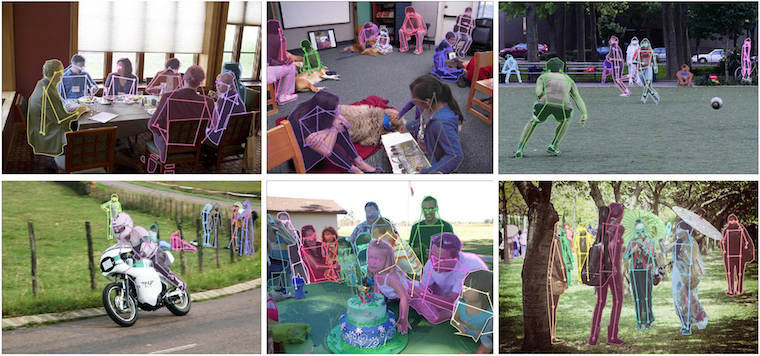
\includegraphics[width=0.75\linewidth]{images/keypointDS1.png}
\end{figure}
}

\end{frame}

% \begin{frame}[fragile]{Data format}

% \scriptsize
% \begin{minted}{json}
% annotation{
%     "keypoints": [x1,y1,v1,...], 
%     "num_keypoints": int, "
%     [cloned]": ...,
% }

% categories[{
%     "keypoints": [str], 
%     "skeleton": [edge], 
%     "[cloned]": ...,
% }]
% \end{minted}

% \verb|[cloned]|: denotes fields copied from object detection annotations defined above.

% \vspace{5mm} 

% {\color{gray}
% % TODO: tldr https://cocodataset.org/#format-data
% The data contains all information about object annotation and two additional fields.\\
% First we have 3k array of keypoints (assuming we have k keypoints) containing position ($x, y$ 0-indexed) and visibility flag ($v\in\{0,1, 2\}$ = \{not labeled, labeled not visible, labeled visible\}). Keypoint is visible if it falls in the object segment.\\
% num\_keypoints is number of detected keypoints\\
% For each category we have field "keypoints" and "skeleton"  
% }
% \end{frame}


\begin{frame}{Data}
Additionally we will use HMDB51 from torchvision to provide videos labeled with actions.

\begin{figure}
    \centering
    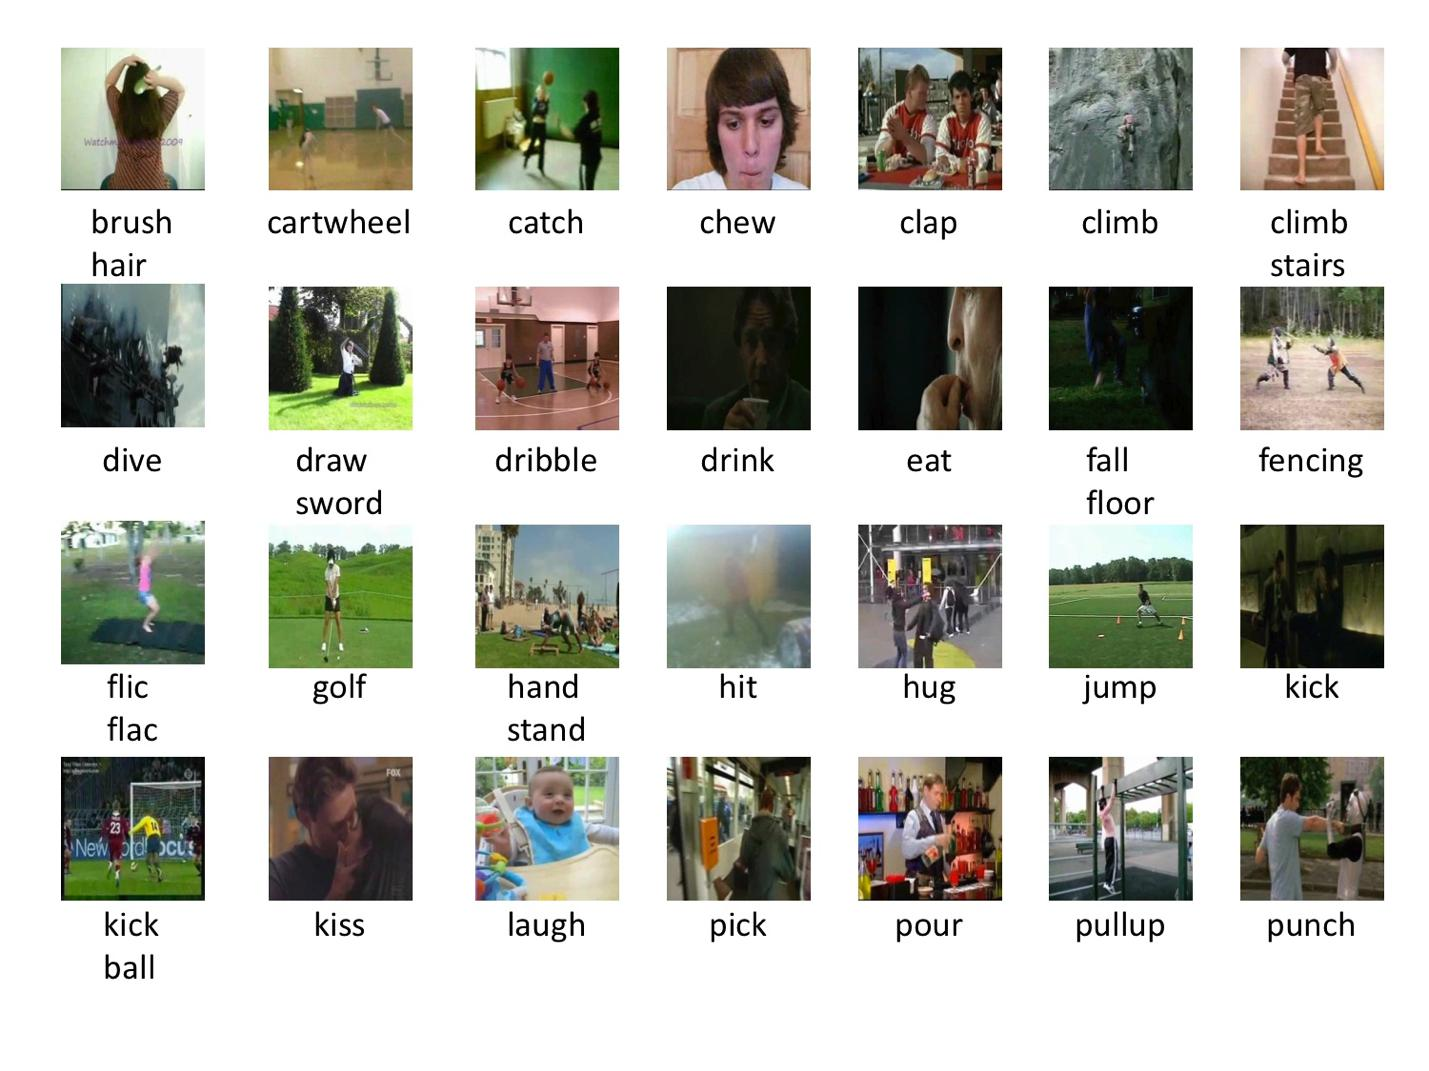
\includegraphics[width=0.7\linewidth]{images/image.png}
\end{figure}

\end{frame}


\begin{frame}{Methods}
The first part of the task is classical Computer Vision problem, so we will use simmilar approach.\\
The second part is classification, but of a video, probably of unknown length. Thats why we are going to use recurrent NN for it.\\
\end{frame}


\begin{frame}{Additional Experiments}
After training the skeletoin-detection model we want to:
\begin{itemize}
    \item Check convolution layers to see what kernels have been trained
    \item Check last convolution layers to see how they react for some input data
    \item Try to extract some images that optimize human features (such as "perfect head")
\end{itemize}
\end{frame}



\end{document}
